\section{Обзор литературы}

% \subsection{Нелинейно-оптические хромофоры и их применение}

% Нелинейные оптические среды~--- это такие среды, в которых вектор поляризации $\mathbf{P}$ зависит от напряженности внешнего электрического поля $\mathbf{E}$ нелинейно:

% \begin{equation}
%     \mathbf{P} = \mathbf{P_0} + \chi^{(1)}_{ij} E_i + \chi^{(2)}_{ijk} E_i E_j + \cdots ,
% \end{equation}

% \noindent где $\chi^{(n)}$~-- n-ый нелинейный коэффициент.\todo{Разобраться с тензорами}

% Такое свойство этих сред позволяет проявляться нелинейными оптическим эффектам: генерации кратных гармоник, сложению частот, генерации разностной частоты и другим многофотонным процессам.

% Нелинейность второго порядка позволяет управлять нелинейными эффектами с помощью внешнего электрического поля~(эффект Поккельса). Она требует отсутствия центра симметрии в молекуле; на практике это достигается использованием асимметричного донорно-акцепторного хромофора. Второй нелинейный коэффициент образца $\chi^{(2)}_{ijk}$ зависит от молекулярной восприимчивости $\beta_{ijk}$ следующим образом:

% \begin{equation}
%     \chi^{(2)} \propto N \beta_{ijk} \langle\cos^3\theta\rangle,
%     \label{eqn:2_nonlinear_coefficient}
% \end{equation}

% \noindent где $N$~--плотность образца (\si{\metre^{-3}}), член $\langle \cos^3\theta\rangle$ соответствует отклонению формы молекулы от сферы. Тогда основной элемент тензора электрооптического эффекта Поккельса $r_{33}$ выражается как:

% \begin{equation}
%     r_{33} = \frac{-2\chi^{(2)}}{\eta^4},
% \end{equation}

% \noindent где $\eta$~--показатель преломления.

% Таким образом, для максимизации нелинейных свойств хромофоров согласно уравнению~\ref{eqn:2_nonlinear_coefficient} необходимо увеличивать как молекулярную восприимчивость $\beta$, которая зависит от структуры хромофора, так и произведение $N\langle \cos^3\theta\rangle$, которое зависит от расположения молекул хромофора в матрице и межмолекулярного взаимодействия~\cite{Dalton2010a}. \todo{Оно надо настолько подробно?}

% Материалы на основе нелинейных донорно-акцепторных хромофоров применяются в электрооптических~(ЭО) модуляторах. Электрооптический модулятор~--- устройство сопряжения между электрическими и оптическими системами связи, позволяющее преобразовывать электрический сигнал в оптический~\cite{2016b}.

% Большинство современных коммерческих образцов ЭО~модуляторов основаны на неорганических нелинейно-оптических материалах, например на ниобате лития. Неорганические НЛО материалы по сравнению с органическими имеют ряд недостатков: низкая нелинейная восприимчивость и, как следствие, высокие значения управляющих напряжений, зависимость НЛО свойств от температуры и ограниченность полосы модулируемого излучения.

% Таким образом, применение органических материалов полимер-хромофор позволяет создавать более эффективные ЭО~модуляторы с использованием методов фотолитографии и микропечати \cite{Han2018}.

\subsection{Сопряженные донорно-акцепторные хромофоры}

Сопряжённые донорно-акцепторные хромофоры представляют большой интерес из-за их электрооптических свойств: система сопряженных двойных связей позволяет образовать низколежащую \ac{lumo} и реализовать внутримолекулярный перенос заряда. Они применяются в таких областях, как органическая электроника, электрооптика, фотовольтаика~\cite{Bures2014a}.

Общая структура донорно-акцепторного хромофора представлена на \ref{fig:D-p-A_chromophores} и включает в себя донорный блок~(\textbf{D}), \chempi-сопряженный мостик~({\Large\chempi}) и акцепторный блок~(\textbf{A}).
\begin{figure}
    \centering
    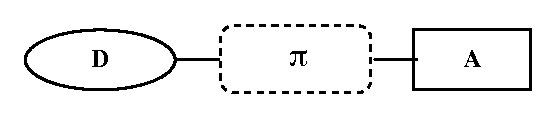
\includegraphics{sections/literature/img/D-p-A_chromophores.eps}
    \caption{Общая структура донорно-акцепторных хромофоров}
    \label{fig:D-p-A_chromophores}
\end{figure}

Внутримолекулярный перенос заряда хорошо заметен при сравнении спектров поглощения анилина, нитробензола, \emph{пара-} и \emph{мета-}нитроанилина~(\ref{fig:UV-nitroaniline}).
В спектре \emph{пара-}нитроанилина присутствует интенсивная полоса переноса заряда из-за сопряжения, присутствующего в молекуле и возможности образования цвиттерионной резонансной структуры.
В спектре \emph{мета-}нитроанилина соответствующая полоса имеет гораздо меньшую интенсивность из-за отсутствия сопряжения между нитрогруппой и аминогруппой~\cite{Bures2014a}.
\begin{figure}
    \centering
    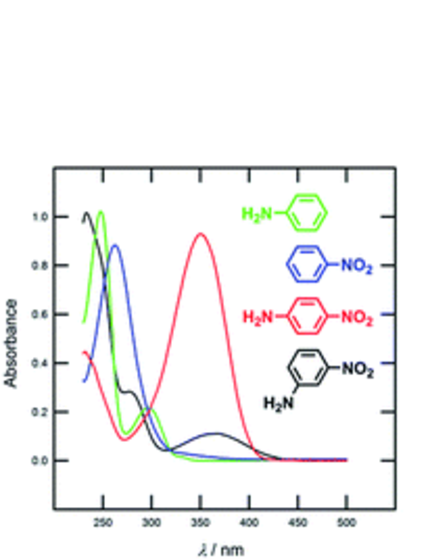
\includegraphics{sections/literature/img/UV-Vis.pdf}
    \caption{Сравнение спектров поглощения анилина, нитробензола, \emph{пара-} и \emph{мета-}нитроанилина~\cite{Bures2014a}}
    \label{fig:UV-nitroaniline}
\end{figure}

Донорно-акцепторные хромофоры могут иметь различные организации: линейную~(диполярную)~~--- \ce{D-\chempi-A}, квадрупольную~--- \ce{D-\chempi-A-\chempi-D} или \ce{A-\chempi-D-\chempi-A}, октапольную~---\ce{(D-\chempi)3-A} или \ce{(A-\chempi)3-D}.
В литературе описаны хромофоры с более редкими структурами, такие как V-образная~\cmpd{V-shape}~\cite{Ramirez2012}, Y-образная~\cite{Hrobarik2011}, H-образная~\cmpd{H-shape}~\cite{Wu2013a} и X-образная~\cmpd{X-shape}~\cite{Chase2011,Bures2007,Zhao2014a}.
\begin{figure}
    \centering
    \begin{overpic}{sections/literature/img/chromophore_shapes.eps}
        \put(18, 5){\cmpd{V-shape}}
        \put(63, 6){\cmpd{X-shape}}
        \put(47, 55){\cmpd{H-shape}}
    \end{overpic}
    \caption{Различные структуры нелинейных хромофоров}
\end{figure}
\FloatBarrier

% \subsubsection{Донорные блоки}
% В качестве доноров в молекулах донорно-акцепторных хромофоров могут использоваться +I/+M заместители~(\ce{OH}, \ce{OR}, \ce{NH2}, \ce{NR2}), электрон-избыточные гетероциклы: производные тиофена~\cite{doi:10.1002/9780470745533.ch1}, метиленпираны~\cite{Gauthier2013}, а также металлоцены~\cite{Long1995,Salman2013}.

% Наиболее распространены донорные блоки на основе диалкил- и диариламинов. 
% Доноры на основе диалкиламинов демонстрируют высокую донорную способность, легкость синтеза и дальнейшей функционализации. 
% Диарилзамещенные амины по сравнению с диалкилзамещенными обладают меньшей донорной способностью из-за делокализации неподеленной пары азота и более сложны в функционализации, однако имеют большую температурную устойчивость~\cite{Dalton2010a}.

% В работах~\cite{2019, Shelkovnikov2019} показано, что в качестве донорных блоков могут быть использованы производные ди- или триарилпиразолинов, которые рассматриваются как циклические аналоги N,N-диалкилпиразолинов.

% \subsubsection{Акцепторные блоки}
% Как акцепторы используются типичные группы с -I/-M эффектом, такие как \ce{CHO}, \ce{NO2}, \ce{CN} и другие. Также используются электрон-дефицитные гетероциклы: (ди)азины~\cite{Achelle2013}, бензотиазолы~\cite{Hrobarik2011}, имидазолы~\cite{Kulhanek2012}, пирролины~\cite{Jang2006}.
% \begin{figure}
%     \centering
%     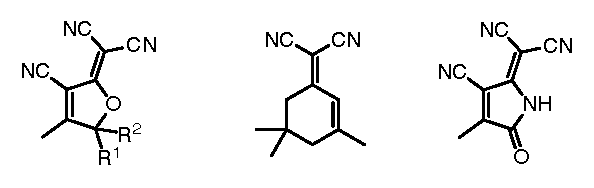
\includegraphics{sections/literature/img/acceptors.eps}
%     \caption{Различные акцепторы~\cite{Dalton2010a}}
%     \label{fig:acceptors}
% \end{figure}

% Дицианоизофорон~\textbf{\cmpd{dicianoisophorone}} был впервые\todo{Впервые ли?} получен Лемке~\cite{Lemke1974} из изофорона~\textbf{\cmpd{isophorone}} и малононитрила

% \begin{scheme}
%     \centering
%     \begin{overpic}{sections/literature/img/dicianoisophoroneLemke.eps}
%         \put(12,10){\textbf{\cmpd{isophorone}}}
%         \put(85,10){\textbf{\cmpd{dicianoisophorone}}}
%     \end{overpic}
%     \caption{Получение дицианоизофорона}
%     \label{sch:dicianoisophoroneLemke}
% \end{scheme}

\subsection{Подходы к синтезу 2-пиразолинов}
2-Пиразолины~(\ref{fig:pyrazoline_structure}) были впервые синтезированы в 19 веке Фишером и Кнёвенагелем реакцией \chemalpha,\chembeta-ненасыщенных альдегидов и кетонов с фенилгидразином при кипячении в уксусной кислоте.

Химия пиразолинов получила развитие в середине XX века в связи с применением арилпиразолинов в качестве оптических отбеливателей и органических сцинтиляторов.
Благодаря их люминисцентным свойствам в настоящее они используются для создания органических светодиодов~(OLED)~\cite{Stakhira2012,Ramkumar2015,Vandana2016}.

Производные пиразолина проявляют биологическую активность, поэтому их синтез представляет большой интерес~\cite{Salian2018, Singh2018,Korablina2016}.
Пиразолины проявляют противомикробную~\cite{Hassan2013}, противодиабетическую~\cite{Ahn2004}, противоэпилептическую~\cite{GunizKucukguzel2000}, антиоксидантную~\cite{Jagadish2013}, противовоспалительную~\cite{Barsoum2006} активность.

\begin{figure}
    \centering
    
\includegraphics{sections/literature/img/pyrazoline_structure.eps}
    \caption{Структура и нумерация атомов 2-пиразолина}
    \label{fig:pyrazoline_structure}
\end{figure}

\subsubsection{Синтез из халконов и гидразинов}

Основным способом синтеза 2-пиразолинов является реакция конденсации халконов с гидразинами. 
Этот подход является достаточно общим, как было показано в работе~\cite{Powers1998}, где таким способом была получена библиотека из \num{7680} 1,3,5-триарилпиразолинов с различными заместителями во всех трех ароматических ядрах.

\begin{scheme}
    \centering
    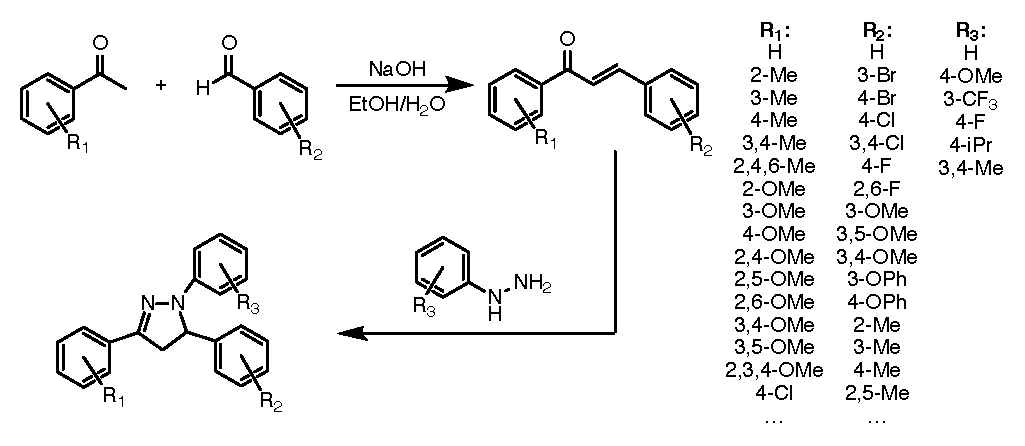
\includegraphics{sections/literature/img/pyrazolines_common.eps}
    \caption{Cинтез триарилпиразолинов с использованием халконов}
\end{scheme}

Халконы представляют собой соединения с двумя электрофильными центрами~--- карбонильной группой и сопряженной связью \ce{C=C}.
Однако в реакциях халконов с гидразинами наблюдается высокая региоселективность~(в отличие от, например, 1,3-дикетонов), в реакцию с атомом азота первой вовлекается карбонильная группа.
Такое поведение обычно объясняют повышенной нуклеофильностью первичного атома азота в замещенных гидразинах по сравнению с вторичным.

Механизм образования пиразолинов~(\ref{sch:pyrazoline_mechanism}) включает в себя образование гидразона и атаку вторичного атома азота на сопряженную двойную связь, замыкающую цикл.
Стадия замыкания цикла является лимитирующей и ее скорость значительно зависит от пространственного и электронного строения гидразона, а также от кислотности среды.

\begin{scheme}
    \centering
    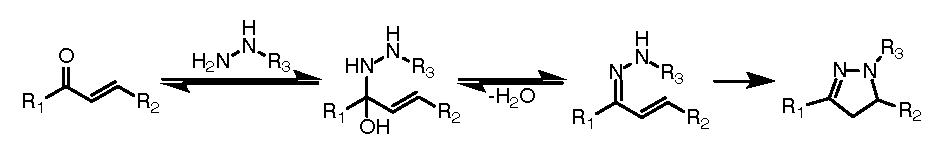
\includegraphics{sections/literature/img/pyrazoline_mechanism.eps}
    \caption{}
    \label{sch:pyrazoline_mechanism}
\end{scheme}

В случае фенилгидразина лимитирующей стадией является дегидратация, а стадия циклизации является быстрой и самопроизвольной.
На ход реакции в наибольшей мере влияет заместитель при карбонильной группе~(\ce{R1}) и его влияние мало зависит от кислотности среды.
Было показано, что реакция фенилгидразина с диарилиденацетонами происходит по фрагменту, содержащему донорную группу~\cite{Chebanov2008}.

Обычно сначала получают халкон конденсацией Кляйзена-Шмидта в основных условиях и вводят его в реакцию с арилгидразином в кислых условиях.
Однако описаны как конденсация в кислых условиях~\cite{Wang2010, Nielsen}, так и циклизация в основных~\cite{Munawar2008, Neudorfer2014, Manyem2007, Patel2004, Singh2014}.

Существует \emph{one-pot} модификация этого метода~(\ref{sch:one-pot}), в этом варианте халкон не выделяется в индивидуальном виде, а сразу же реагирует с фенилгидразином, присутствующим в реакционной смеси.
При этом реакция проводится целиком в основной среде~\cite{Farooq2020}.

\begin{scheme}
    \centering
    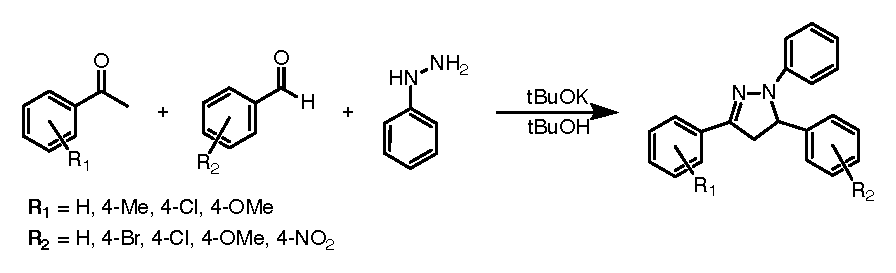
\includegraphics{sections/literature/img/one-pot.eps}
    \caption{}
    \label{sch:one-pot}
\end{scheme}

В недавнее время были предприняты попытки проводить реакцию в более экологичных условиях, используя в качестве циклизующего агента вольфрамсерную кислоту~\cite{Rahmatzadeh2015} и целлюлозосульфоновую кислоту~\cite{Daneshfar2015}.
Также в качестве экологически чистых методов исследовались синтез в водных растворах~\cite{Markovic2015}, механохимический синтез~\cite{Zangade2013}, микроволновый синтез~\cite{Adhikari2012} и ультразвуковой синтез~\cite{Shelke2012}. \todo{дописать?}

Получение полифторированных триарилпиразолинов несет в себе больше сложностей: в случае разных заместителей халкона часто не удается подобрать условия реакции таким образом, чтобы получать селективно один региоизомер~--- образуется смесь продуктов с разными заместителями в положениях 3 и 5.
Так, в работе~\cite{2010} изучается взаимодействие фенилгидразина с халконами, с одним полифторированным кольцом~(\ref{sch:polyflouro_isomers}).

\begin{scheme}
    \centering
    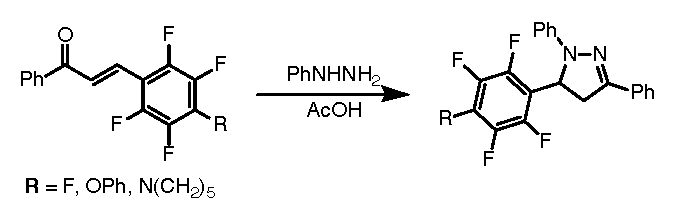
\includegraphics{sections/literature/img/polyflouro_isomers.eps}
    \caption{Образование двух региоизомеров 2-пиразолина}
    \label{sch:polyflouro_isomers}
\end{scheme}

Было обнаружено, что халконы с акцепторным заместителем при двойной связи при кипячении образуют один региоизомер пиразолина, а халконы с акцепторным заместителем при карбонильной группе~--- два региоизомера в сравнимых количествах.
Это можно объяснить большим различием \chemsigma\textsuperscript{*}-констант заместителей при двойной связи~(\ce{C6F5CO} и \ce{Ph}), из-за чего усиливается электрофильный характер \chembeta-атома углерода, что дает возможность нуклеофильной атаки фенилгидразина как по карбонильной группе, так и по двойной связи.

\subsubsection{Синтез из аналогов халконов}
Сопряженные енины можно считать аналогами халконов, поскольку при гидратации тройной связи образуется соответствующий кетон.
В работе~\cite{Patil2011} была исследована реакция циклизации арилгидразинов с 1,3-енинами при катализе различными метал-содержащими реагентами~(\ref{sch:enine_synthesis}).
Было показано, что при микроволновом облучении смеси сопряженных енинов с арилгидразинами в присутствии~\ce{Zn(OTf)2} наблюдается наилучший выход соответствующих пиразолинов.
В ходе реакции происходит двойное гидроаминирование сначала тройной, а потом двойной связи.

\begin{scheme}
    \centering
    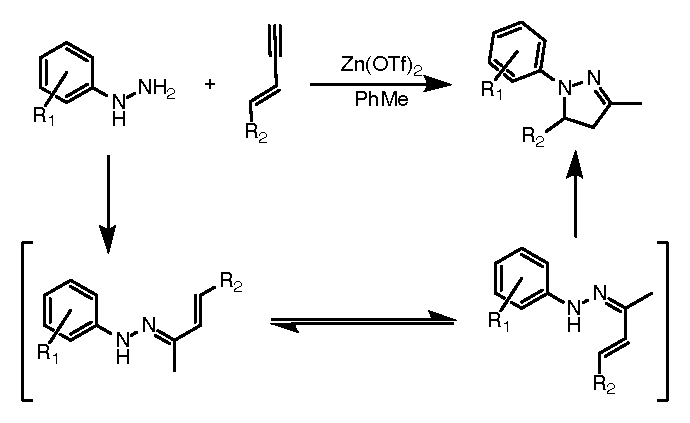
\includegraphics{sections/literature/img/enine_synthesis.eps}
    \caption{}
    \label{sch:enine_synthesis}
\end{scheme}

Некоторые пропаргиловые спирты способны вступать в перегруппировку с образованием халконов.
При исследовании реакции сочетания Соногаширы вторичных пропаргиловых спиртов с арилгалогенидами было обнаружено, что при наличии акцпторных заместителей в арилгалогениде такая перегруппировка может происходить под действием триэтиламина, который присутствует в реакционной смеси~(\ref{sch:sonogashira})~\cite{Muller2000}.

\begin{scheme}
    \centering
    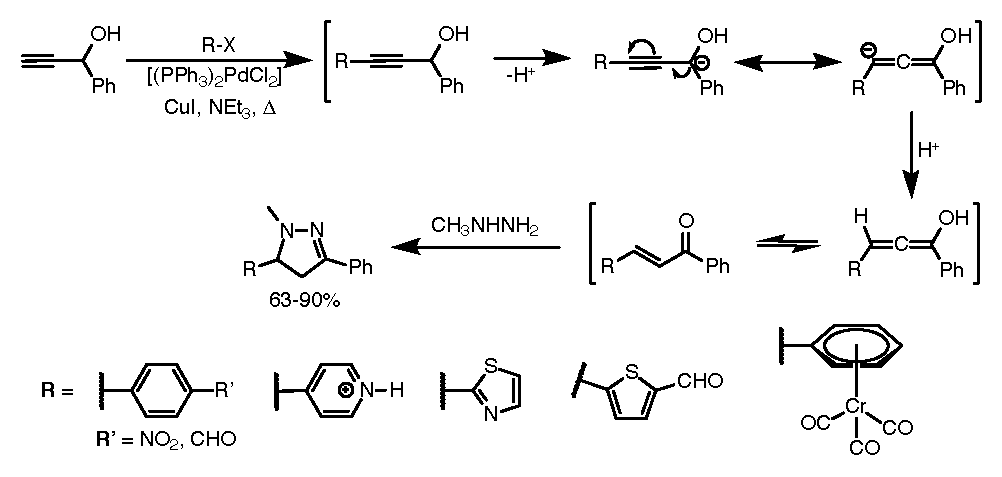
\includegraphics{sections/literature/img/sonogashira.eps}
    \caption{}
    \label{sch:sonogashira}
\end{scheme}

Пропаргиловые спирты, не содержащие акцепторных заместителей, также способны вступать в эту перегруппировку, однако в более жестких условиях.
В работе~\cite{Wang2014} была разработана и оптимизирована методика синтеза пиразолинов из пропаргиловых спиртов и арилгидразинов в присутствии~\ce{tBuOK}~(\ref{sch:propargyl}).

\begin{scheme}
    \centering
    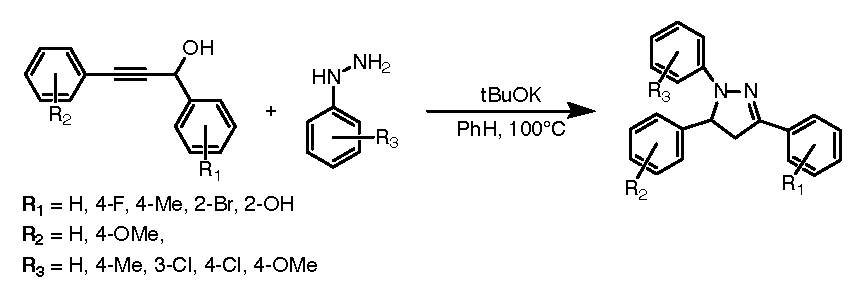
\includegraphics{sections/literature/img/propargyl.eps}
    \caption{}
    \label{sch:propargyl}
\end{scheme}

\subsubsection{Синтез [3 + 2] циклоприсоединением}

Второй способ синтеза пиразолинов использует [3 + 2] циклоприсоединение илидов азометиновых иминов~\textbf{\cmpd{azomethine}} к алкинам. Циклоприсоединение 1,3-диполей к диполярофилам является удобным способом получения пятичленных циклов. Наиболее известным примером таких реакций является присоединение азидов к алкинам. Считается, что [3 + 2] циклоприсоединение идет по согласованному механизму. Использование комплексов металлов с хиральными лигандами в качестве катализаторов позволяет селективно получать энантиомерно чистые пиразолины. Циклоприсоединение илидов азометиновых иминов к алкенам дает полностью насыщенные аналоги пиразолинов~--- пиразолидины~\cite{Groselj2018}. \todo{Какой-то несогласованный абзац}

\begin{scheme}
    \centering
    \begin{overpic}{sections/literature/img/pyrazolines_cycloaddition.eps}
        \put(35,2){\textbf{\cmpd{azomethine}}}
    \end{overpic}
    \caption{Синтез триарилпиразолинов с использовнием [3 + 2] циклоприсоединения}
\end{scheme}


Азометиновые имиды можно представить в виде четырех резонансных структур~(\ref{fig:azomethine_resonance})~--- двух иминных и двух диазониевых. Чаще всего их изображают с зарядами, локализованными на атомах азота, такое распределение зарядов соотносится с квантовомеханическими расчетами~\cite{Groselj2018}.

\begin{figure}
    \centering
    \begin{overpic}{sections/literature/img/azomethine_resonance.eps}
    \end{overpic}
    \caption{Резонансные структуры илидов азометиновых иминов}
    \label{fig:azomethine_resonance}
\end{figure}

% Существует несколько способов получения илидов азометиновых иминов в основном \ac{insitu}, включающие генерацию из гидразонов~\textbf{\cmpd{hydrazone}} с последующим [3 + 2] циклоприсоединением, генерацию из енгидразинов~\textbf{\cmpd{enhydrazine}}, взаимодействие 1,2-дизамещенных гидразинов~\textbf{\cmpd{carbene}} с карбенами, взаимодействие азосоединений~\textbf{\cmpd{azo}} с диазоалканами~\textbf{\cmpd{diazo}}, окисление N,N,N\chemprime-тризамещенных гидразинов~\textbf{\cmpd{oxidation}}, 1,4-силатропный сдвиг в \chemalpha-силилнитрозаминах и \chemalpha-силилнитрозамидах~\textbf{\cmpd{silyl}} и метатезис 1,2-диарилдиазен-1-оксидов~\textbf{\cmpd{metathezis}}~\cite{Padwa2005}.

% \begin{scheme}
%     \centering
%     \begin{overpic}{sections/literature/img/azomethine_generation.eps}
%         \put(6, 44){\textbf{\cmpd{hydrazone}}}
%         \put(56, 44){\textbf{\cmpd{enhydrazine}}}
%         \put(6, 29){\textbf{\cmpd{carbene}}}
%         \put(62, 29){\textbf{\cmpd{silyl}}}
%         \put(6, 15){\textbf{\cmpd{oxidation}}}
%         \put(49, 16){\textbf{\cmpd{diazo}}}
%         \put(65, 16){\textbf{\cmpd{azo}}}
%         \put(22, 0){\textbf{\cmpd{metathezis}}}
%     \end{overpic}
%     \caption{Различные способы получения илидов азометиновых имидов}
% \end{scheme}

Синтез пиразолинов, исходя из ациклических илидов азометиновых иминов, получаемых \ac{insitu}, был подробно изучен в работе~\cite{Hashimoto2013}. В этой работе было синтезировано более \num{18} пиразолинов и проведена оптимизация условий реакции: было изучено влияние различных солей \ce{Cu(I)} и заместителей лигандов и субстратов.

\begin{scheme}
    \centering
    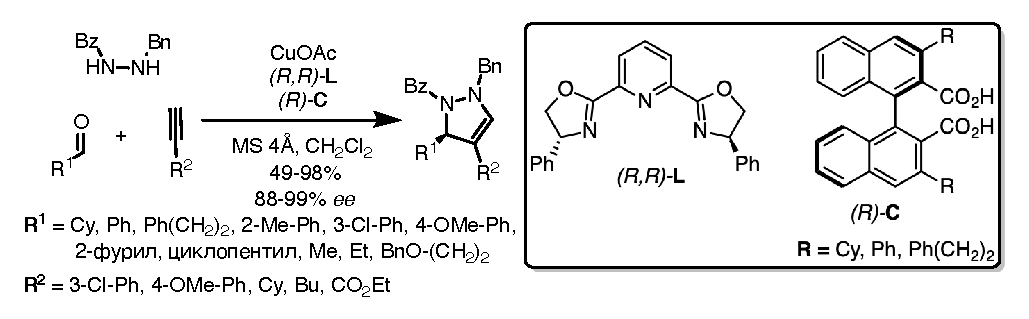
\includegraphics{sections/literature/img/cycloaddition_example.eps}
    \caption{Энантиоселективный синтез пиразолинов с использованием [3 + 2] циклоприсоединения~\cite{Hashimoto2013}}
\end{scheme}
\FloatBarrier

\subsection{Синтез других изомеров пиразолина}

\subsubsection{Синтез 1-пиразолинов}
В работах~\cite{Baldwin1990, Mish1997, Simovic2007, Sun2013} описан синтез 1-пиразолинов из соединений, содержащих двойную свзь. и производных диазометана. 
Обычно 1-пиразолины нестабильны и склонны к перегруппировке в соответствующие 2-пиразолины~(\ref{sch:1-pyrazoline-TMS.eps}), что было показано в~\cite{Mish1997, Simovic2007}.

\begin{scheme}
    \centering
    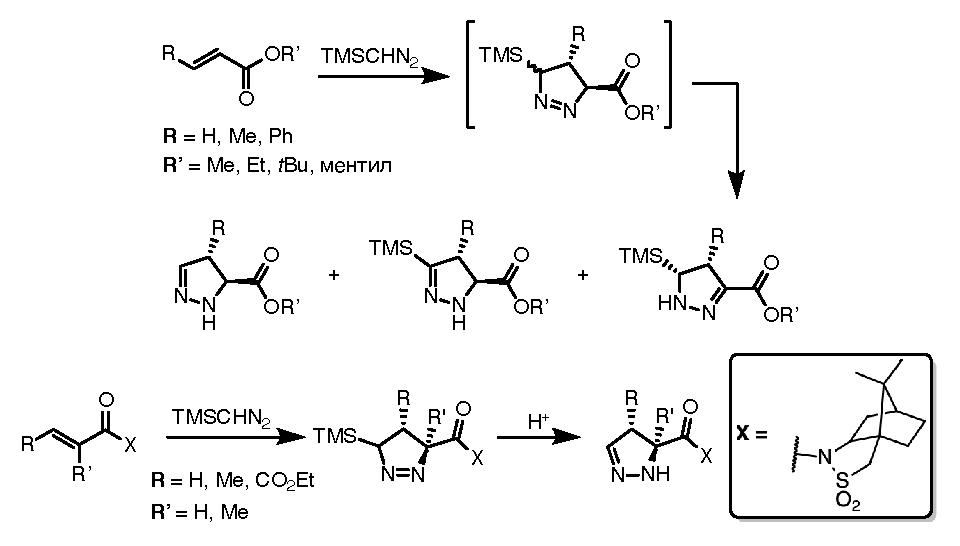
\includegraphics{sections/literature/img/1-pyrazoline-TMS.eps}
    \caption{}
    \label{sch:1-pyrazoline-TMS.eps}
\end{scheme}


Тетразамещенные 1-пиразолины полученные в работе~\cite{Sun2013} из защищенных аддуктов Бейлиса-Хиллмана и ацилдиазометанов имеют по два заместителя в положениях 3 и 5, и поэтому не могут перегруппироваться в соответствующие 2-пиразолины~(\ref{sch:1-pyrazoline-4}).

\begin{scheme}
    \centering
    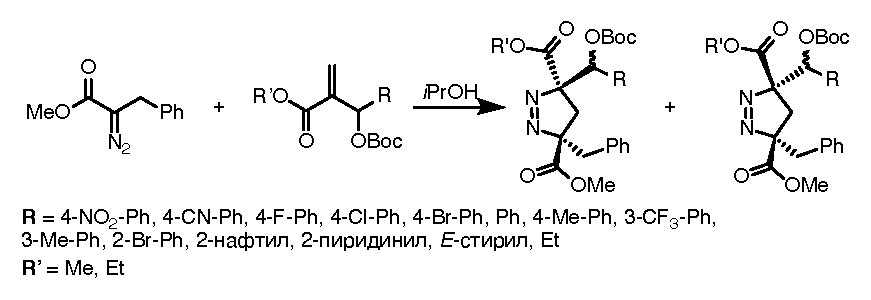
\includegraphics{sections/literature/img/1-pyrazoline-4.eps}
    \caption{}
    \label{sch:1-pyrazoline-4}
\end{scheme}


В~\cite{Baldwin1990} взаимодействием цефалоспорина содержащего экзоциклическую связь и диазометана был получен сравнительно стабильный 1-пиразолин.
Полученное соединение не подвергается никакому изменение при кипячении в толуоле в течение восьми дней, но в диметилформамиде дает смесь двух продуктов: циклопропана, соответствующего присоединению карбена по исходной двойной связи, и винильного производного~(\ref{sch:cefalosporine}). 

\begin{scheme}
    \centering
    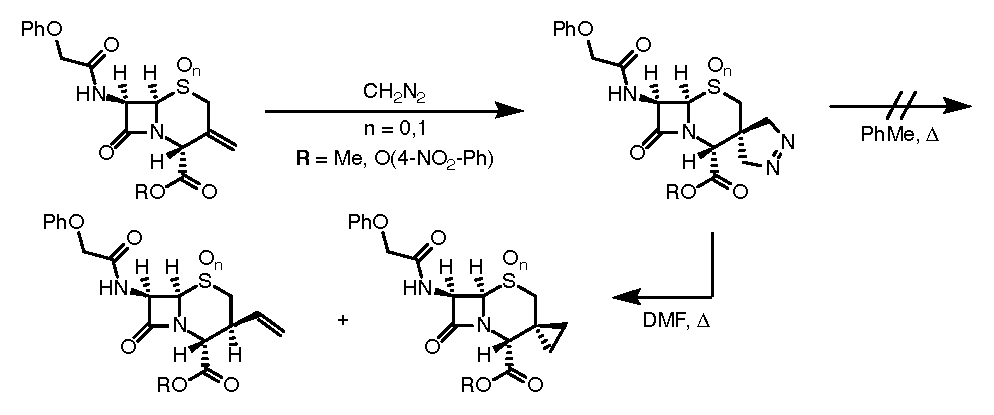
\includegraphics{sections/literature/img/cefalosporine.eps}
    \caption{}
    \label{sch:cefalosporine}
\end{scheme}


\subsubsection{Синтез 3-пиразолинов}
3-Пиразолины существуют только в 1,2-дизамещенном виде за исключением нескольких примеров. 
Для 3-пиразолинов незамещенных по обоим атомам азота существует лишь один пример описанный в~\cite{Misani1956}, 3-пиразолины, замещенные только по одному атому азота несколько более известны~\cite{Takamizawa1963, Takamizawa1965, Armstrong1973, Burger1979}. 
Главным способом синтеза 1,2-замещенных 3-пиразолинов является реакция Манниха симметричных дизамещенных гидразинов с формальдегидом и кетоном. Получающееся основание Манниха вступает во внутримолекулярную циклизацию с образованием соответствующего 3-пиразолина~(\ref{sch:3-pyrazoline}). 
Позиция двойной связи была подтверждена с помощью ИК-спектроскопии, показавшей наличие сопряжения между двойной связью пиразолина и бензольным кольцом.

\begin{scheme}
    \centering
    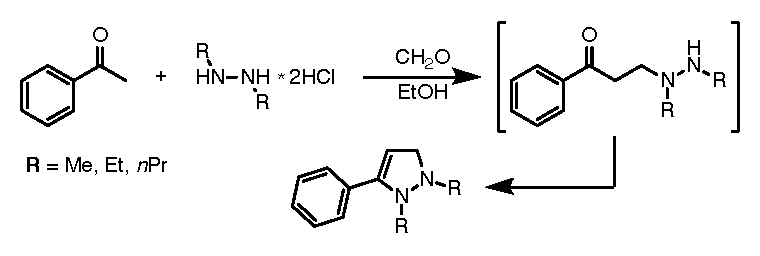
\includegraphics{sections/literature/img/3-pyrazoline.eps}
    \caption{}
    \label{sch:3-pyrazoline}
\end{scheme}

Конденсация гидразида фталевой кислоты с коричным альдегидом дает региоизомерные 3-пиразолины~(\ref{sch:3-pyrazoline_isomer}), которые при гидролизе превращиются в соответсующие 2-пиразолины.
Образование 3-пиразолина было подтверждено с помощью расщепления молекулы и элементого анализа~\cite{Chemistry1967}.

\begin{scheme}
    \centering
    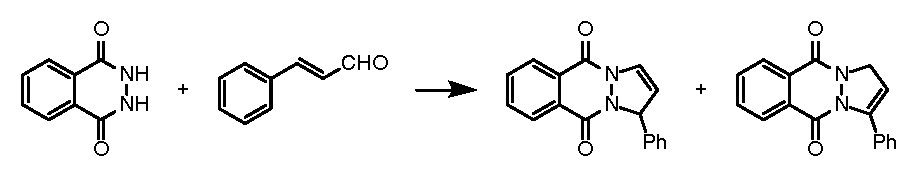
\includegraphics{sections/literature/img/3-pyrazoline_isomer.eps}
    \caption{}
    \label{sch:3-pyrazoline_isomer}
\end{scheme}

\subsection{Реакции пиразолинов}

\subsubsection{Реакции окисления}
Пиразолины неустойчивы к окислению~--- они могут быть переведены в соответствующие пиразолы действием различных окислителей~(\ref{sch:pyrazoline_ox}).
При этом возможно как стехимометрическое окисление~\cite{Zolfigol2004, Dodwadmath1935, Gladstone1966, Auwers1927, Singh1997, Walker1967}, так и каталитическое~\cite{Nakamichi2002, Kojima2016, Shah1978}.

\begin{scheme}
    \centering
    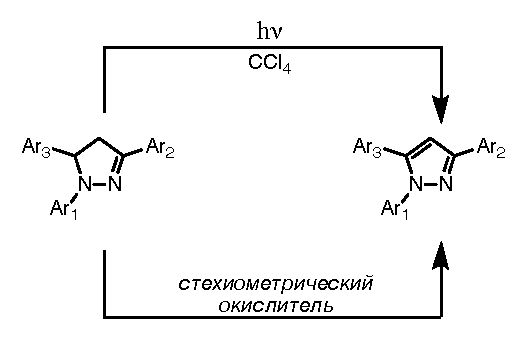
\includegraphics{sections/literature/img/pyrazoline_ox.eps}
    \caption{Окисление пиразолинов в пиразолы}
    \label{sch:pyrazoline_ox}
\end{scheme}

Также описано окисление пиразолинов в хлорированных растворителях~(1,2-дихлорэтан и \ce{CCl4}) под действием видимого света.
В этом случае в качестве окислителя выступает растворитель.
Для этой реакции в работах~\cite{Annes2019,Traven2016} был предложен механизм~(\ref{sch:light_oxidation}), включающий фотовозбуждение молекулы приразолина, перенос электрона на молекулу растворителя и дальнейшие превращения получившегося катион-радикала.

\begin{scheme}
    \centering
    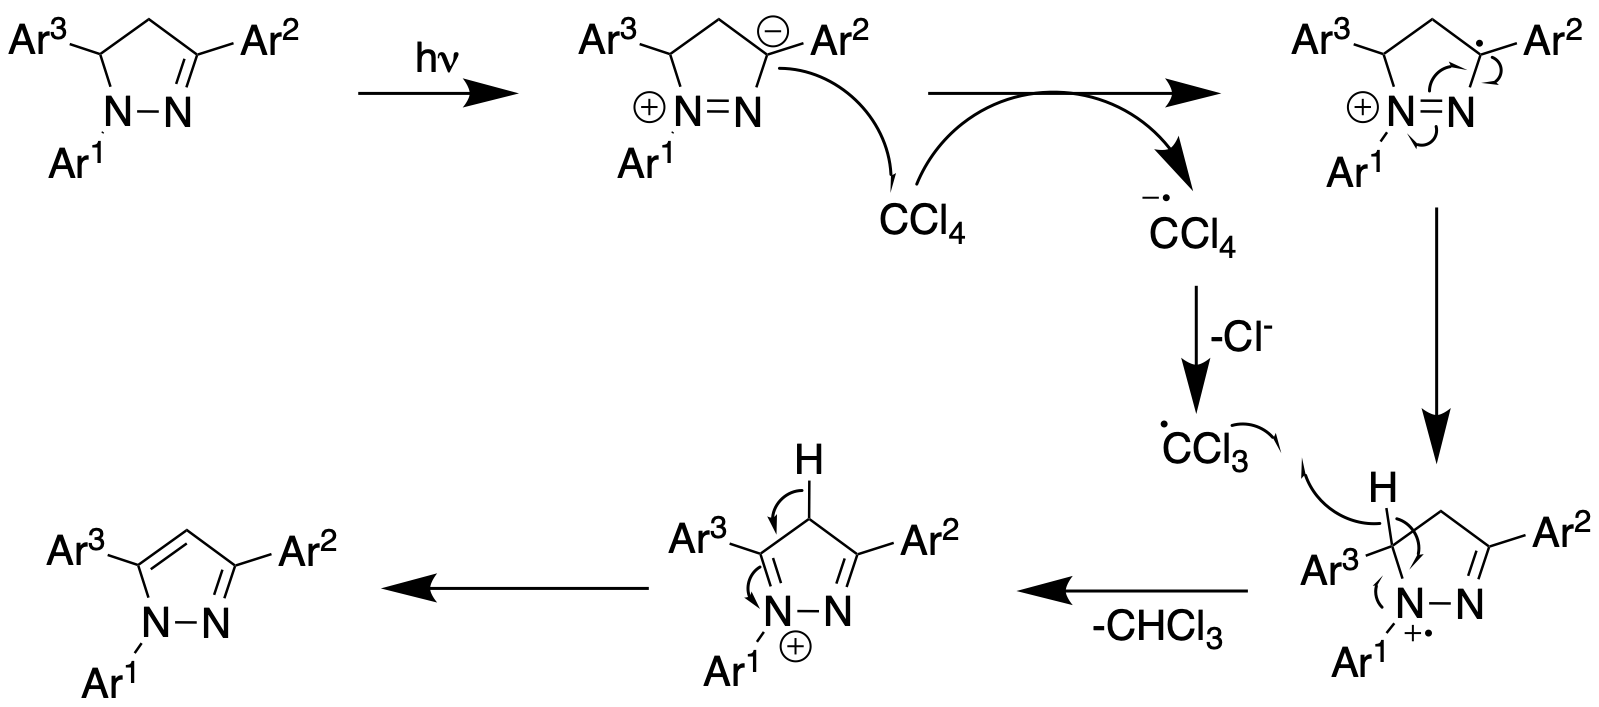
\includegraphics{sections/literature/img/photooxidation.png}
    \caption{Предполагаемый механизм окисления пиразолинов под воздействием света }
    \label{sch:light_oxidation}
\end{scheme}
Радкикальный характер этой реакции подтверждатеся тем, что добавление в реакционную смесь радикальных ингибиторов замедляют реакцию.
Однако полного ингибирования не наблюдается, поскольку стадия образования пиразолиниевого радикала не является лимитирующей~\cite{Traven2016}.

Надкислоты \todo{Перкислоты?} (надуксусная и надбензойная) окисляют 1-пиразолины в соответствующие N-оксиды~(\ref{sch:peracid_ox}).

\begin{scheme}
    \centering
    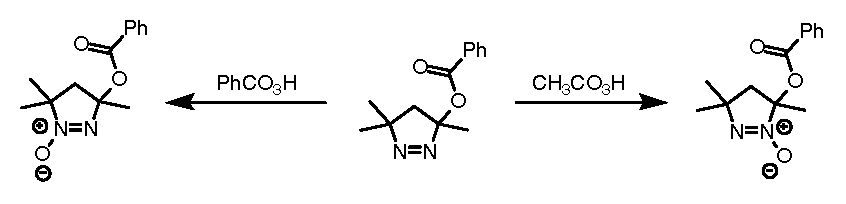
\includegraphics{sections/literature/img/peracid_ox.eps}
    \caption{}
    \label{sch:peracid_ox}
\end{scheme}

 \subsubsection{Реакции восстановления}
Двойная связь \ce{C=N} в пиразолинах может быть восстановлена типичными реагентами~--- комплексными гидридами. В работах~\cite{Jakob2010, DeLosSantos2008a} авторы использовали триэтилборгидрид лития в тетрагидрофуране, а в~\cite{Mish1997a}~--- цианоборгидрид натрия в уксусной кислоте~(\ref{sch:hydride_reduction}).
В каждом случае было испробовано несколько восстановителей и выбор конкретного~--- баланс между выходом целевого продукта и образованием побочных продуктов~(например, деацилирования).

\begin{scheme}
    \centering
    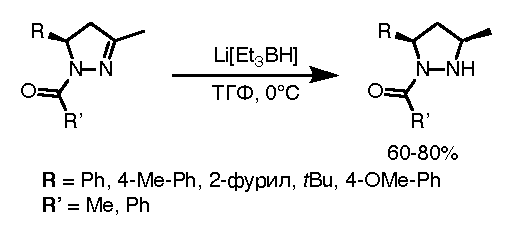
\includegraphics{sections/literature/img/hydride_reduction.eps}
    \caption{}
    \label{sch:hydride_reduction}
\end{scheme}

В других условиях пиразолины можно восстановить с расщеплением связи \ce{N-N}. 
Восстановление пиразолинов натрием в этаноле можно использовать для получения 1,3-диаминозамещенных пропанов~\cite{Chemistry1967}.
Для получения 1,3-диаминокарбоновых кислот в работе~\cite{Carter1949} использовали восстановление водородом под давлением на никеле Ренея~(\ref{sch:hydrogen_reduction}).

\begin{scheme}
    \centering
    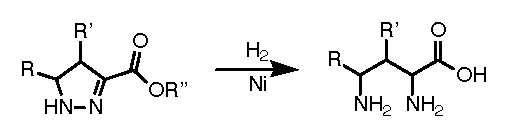
\includegraphics{sections/literature/img/hydrogen_reduction.eps}
    \caption{}
    \label{sch:hydrogen_reduction}
\end{scheme}